\documentclass[10pt,a4paper]{article}
\usepackage[latin1]{inputenc}
\usepackage{amsmath}
\usepackage{amsfonts}
\usepackage{amssymb}
\usepackage{graphicx}
\usepackage{float}
\author{Michele De Vita}
\begin{document}
	\begin{enumerate}
		\item If \textit{age} increase from 25 to 26 when all other variables are the same we have an increase of \textit{ahe} of 0.31. The same for 33 to 34.
		\item  If \textit{age} increase from 25 to 26 when all other variables are the same we have an increase of \textit{ahe} of $ 2\% $. The same for 33 to 34.
		\item In this case has no sense explain the \textit{age} increase from 25 to 26 because we used a log-log scale that explain the increase by $ 1\% $ of age and not by $ 1 $ unit. If we want to interpreter the coefficient before $ age $ we can say that if age increase by $ 1\% $,  $ ahe $  increase by $ 0.006369 $
		\item Since when $ age  $ increase by one the variable $ age^2 $ also increase we cannot interpreter the coefficient before $ age $
		\item Between the 3 and 2 we prefer the 2 because the explain the increase of $ age $ by 1 $ unit $ instead of $ 1\% $ 
		\item We prefer the 2 because the 4 with $ age^2 $ doesn't explain anything more than 2
		\item We prefer the 3 for the same reason of the point 5 of this exercise
		\item 
		If we see the first two plots are very similar, maybe the second line is a little bit curved while the third with $ age^2 $ is very curved at the end.
		The form of the plots for the female with bachelor are basically the same except for the range of values of y that is between $ 2.50 - 2.70 $ in contrast to $ 2.32 - 2.5 $ for the male with high school
		\begin{figure}[H]
			\centering
			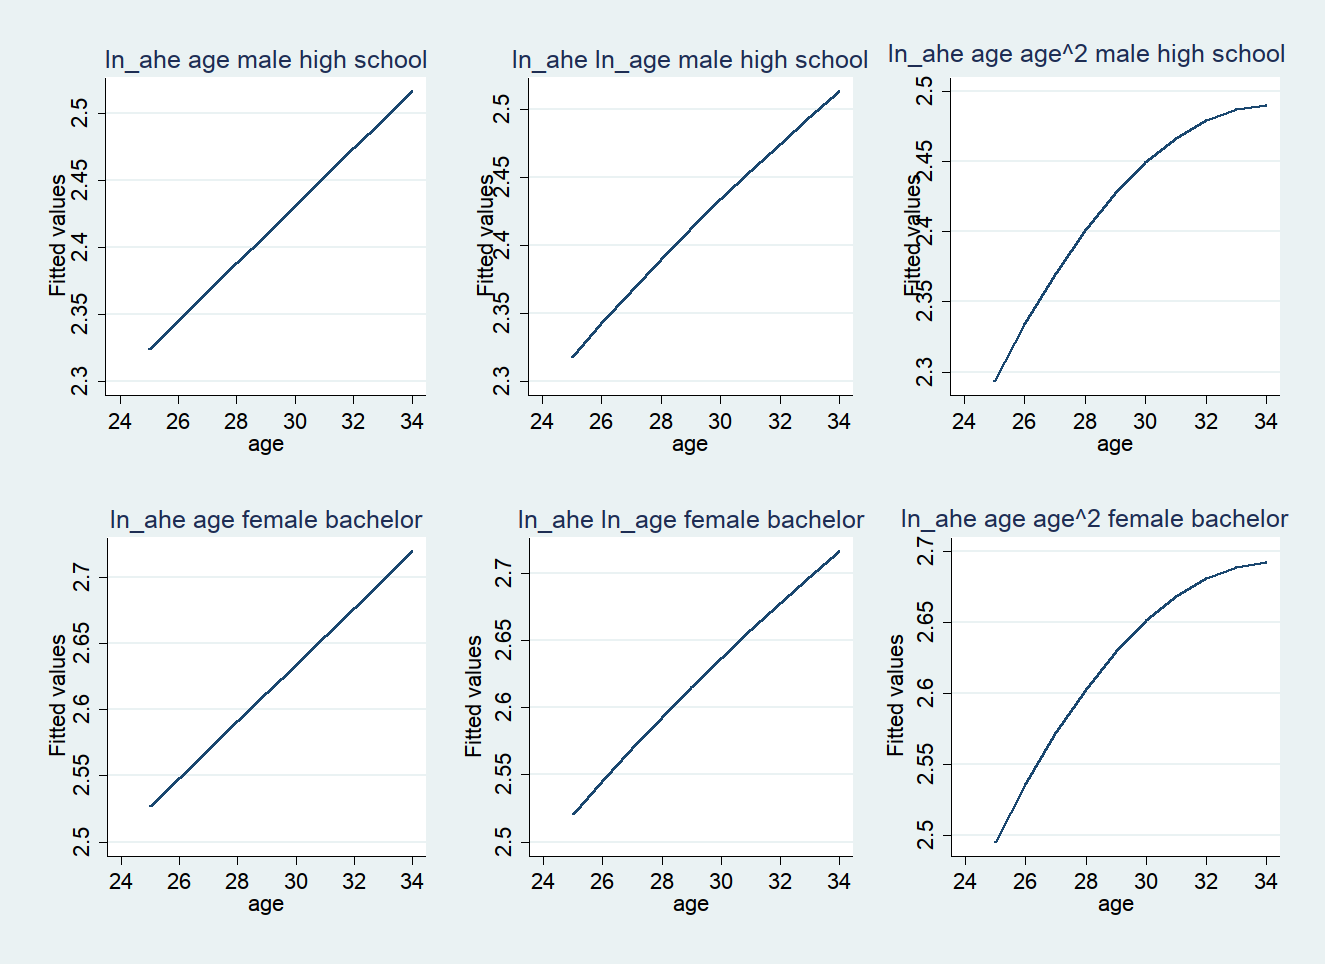
\includegraphics[width=0.7\linewidth]{plot_6_regressions}
		\end{figure}
	\item The interaction coefficient say that if we have two $ female $ with the same age, one with $ bachelor $ and one without, the first have an increase of $ ahe $ by $ 0.345 + 0.084 = 0.43 = 43\% $ .\\
	If we increase by one the $ age $  		
	Jane has a $ \ln(AHE) = 2.63 $ and $ AHE = 13.92 $ while Alexis has a $ \ln(AHE) = 2.20 $ and a $ AHE = 9.05 $. The difference between the two female is $ 2.63 - 2.20 = 0.43 $ that is exactly the interpretation given before.
	Bob has a $ \ln(AHE) = 2.77 $ and $ AHE = 15.95 $ while Jim has a $ \ln(AHE) = 2.421 $ and a $ AHE = 11.26 $. The difference between the two female is $ 2.77 - 2.421 = 0.349 $ that is exactly the bachelor coefficient but without the interaction because $ female = 0 $
	\item First we centre the age values. Then making a regression with the $ age\_center, female $ and the interaction between the last two, we obtain a coefficient equal to $ -0.0070067 $ and a p-value of $  0.124 $,  so there isn't statistical significance for this value then we can't use this value for regression. In conclusion we can say that there isn't a difference on earning between male and female in relation to age
	\item We used the age centred in the mean calculated in the latter exercise. In this case the regression use the variables  $ age\_center, bachelor $ and the interaction between the last two. The coefficient of the interaction is equal to $ 0.00469 $ with a $ p-value = 0.272 $, so also in this case we haven't enough statistical significance to use this value, then we can't assert that there is an effect between $ age $ and $ bachelor $ variables in relation to earning
	\end{enumerate}
\end{document}